\documentclass[sigplan]{acmart}

\settopmatter{printacmref=false} % Removes citation information below abstract
\renewcommand\footnotetextcopyrightpermission[1]{} % removes footnote with conference information in first column
\pagestyle{plain} % removes running headers

\usepackage[english]{babel}
\usepackage{listings}
\usepackage{url}
\usepackage{amsmath,amsthm}
\usepackage{amsfonts}
\usepackage{amssymb}

\begin{document}

\title{Optimizing Cholesky Factorization \\with Intel AVX insructions}

\author{Oleksandr Zaytsev}
\affiliation{%
  \institution{Ukrainian Catholic University\\
  Faculty of Applied Sciences}
  \city{Lviv}
  \state{Ukraine}
}
\email{oleks@ucu.edu.ua}

\begin{abstract}
Software packages like R call native functions highly optimized native libraries like LAPACK, BLAS or Intel MKL. As of this time only MKL library makes use of AVX instructions of Intel processors, which gives it an amazing advantage over  competitors.

In this work I demonstrate how AVX instructions can be used to speed up the execution of widely used numerical algorithms, using Cholesky factorization as an example. This algorithm was chosen because of its simplicity and wide range of applications.
\end{abstract}

\keywords{SIMD, AVX, parallel algorithms, numerical methods, Cholesky factorization}

\maketitle

\section{Introduction}
Intel Advanced Vector Extensions (Intel AVX) is a set of instructions for doing Single Instruction Multiple Data (SIMD) operations on Intel architecture CPU\cite{Lomont}. These instructions allow processing of multiple pieces of data in a single step by performing a simple operation on a small block of single (32-bit) or double-precision (64-bit) floating point values simultaneously. We will be working with 256-bit AVX instructions that work on a packs of 4 double-precision values. Therefore, for example, if we want to add two vectors of 8 elements, we can do it in 2 ticks.

\subsection{Cholesky Factorization}
Every symmetric positive-definite matrix $A$ can be decomposed into the product

\[ A = LL^\top \]

We can think of above equality as of the system of equations with unknowns $l_{ij}$. By solving this system we obtain the formula for the entries of $L$:

\[
    \begin{cases}
        L_{jj} = \sqrt{A_{jj} - \sum_{k=1}^{j-1}L_{jk}^2} \\
        L_{ij} = \frac{1}{L_{jj}} \bigg( A_{ij} - \sum_{k=1}^{j-1}L_{ik}L_{jk} \bigg)
    \end{cases}
\]

Where $L$ is a lower-triandular matrix.

Cholesky factorization simplifies the problem of solving systems of linear equations $Ax = b$ with symmeric positive-definite matrix $A$ by first solving the triangular system $Ly = b$ and then $L^\top x = y$.

There are two versions of iterative Cholesky factorization:

\begin{itemize}
	\item \textbf{Cholesky-Banachiewicz algorithm} -  iterates the matrix row by row
	\item \textbf{Cholesky-Crout algorithm} - iterates the matrix column by column
\end{itemize}

In this work I will be focusing on Cholesky-Banachiewicz factorization.

\section{Data generation}
\label{data}

I used R to generate 6 symmetric positive-definite matrices with real-value entries. The matrices are square and have the following $250, 500, 1000, 2500, 5000, 7500$ rows respectively. These matrices are then stored in binary files and loaded by other modules of this project.

I chose the approach of pre-generated matrices as opposed to the idea of generating a new matrix for each experiment, as it was done in \cite{Tarasconi}, because this way the measurements will be more accurate. I compare the performance of two algorithms on exactly the same input.

\section{Implementation}
There are three parts in the algorithm that can be parallelized:

\begin{enumerate}
\item Inner product of two rows
\item Subtraction of inner product from each element of the row
\item Division by diagonal elements
\end{enumerate}

\subsection{Inner product}

Inner product \texttt{L[i][k] * L[j][k]} in this algorithm does not have any side effects or complex dependencies can be easily extracted from the algorithm and parallelized. We iterate over the batches of 4 elements in each array and perform the following step to multiply them and sum up the results.

\lstset {language=C++}
\begin{lstlisting}
double sum;
__m256d ax = _mm256_loadu_pd(&a[0]);
__m256d bx = _mm256_loadu_pd(&b[0]);
__m256d cx = _mm256_mul_pd(ax, bx);
__m256d hsum = _mm256_add_pd(cx,
    _mm256_permute2f128_pd(cx, cx, 0x1));
_mm_store_sd(&sum,
    _mm_hadd_pd(
        _mm256_castpd256_pd128(hsum),
        _mm256_castpd256_pd128(hsum)));
\end{lstlisting}

We start by loading 256-bits (composed of 4 packed double-precision (64-bit) floating-point elements) from array \texttt{a} into the YMM registers. We do the same for the 4 values from \texttt{b}. Then we perform elementwise multiplication of the two vectors and sum the values of the resulting vector into a scalar.

Intrinsic \texttt{\_mm256\_castpd256\_pd128} is only used for compilation and does not generate any instructions, thus it has zero latency. \texttt{\_mm\_store\_sd} is an SSE2 instruction that stores the lower double-precision floating-point element into memory.

You can see the results of this parallelization in section \ref{exp-res} where I describe the results of my experiments.

\subsection{Further AVX optimization}

Having successfully parallelized the inner product I tried doing the same for other two parallelizable parts of the algoritm mentioned at the beginning of this section. Parallelizing the subtraction did not produce better results. The possible reason for that is the cost of storing sum on each step in order to use it later and the relatively small size of vectors on the first iterations (matrix is triangular).

As for division, it might really benefit from parallelization (as we know, division is a very costly operation) but for that we must choose a different data structure. We store elements of a matrix in a two-dimensional array, which means that the diagonal elements are not located close to each other in the memory. Choosing another data structure would allow us to store the lower triangular elements and diagonal in two different arrays (upper triangular elements would not be stored at all and it would also reduce the memory requirements). This way we could pass the array of diagonal elements to AVX intrinsics parallelize the division. However, this it out of the scope of my project.

\subsection{Multithreading}

In addition to parallelizing inner product over 4 YMM registers, I have tried splitting arrays \texttt{a} and \texttt{b} in two multiplying them separately in two differend POSIX threads. This resulted in much slower execution due to the small size of arrays. Inner product by itself is a fast operation even in its sequential form. In order for the speedup of multithreaded execution to be higher then the latency of creating two threads, we need to multiply arrays that have at least several million elements. In our case the largest arrays we are multiplying have 7500 elements, which means that the cost of creating threads several thousand times (we perform inner product on each row) is much higher than the gain from parallelization.

\section{Experimental results}
\label{exp-res}

I have compared the execution time of sequential Cholesky-Banachiewicz factorization algorithm and its optimized version with AVX instructions on the 6 matrices described in section \ref{data}. In order to get more accurate time measurements I ran each algorithm 10 times on every matrix (making it 60 executions for each method) and visualized the mean of execution time. You can see the results on the following visualization. The line is the mean elapsed time and the error bars show how this time was deviating from the mean across different executions.

\begin{figure}[H]
  \begin{center}
  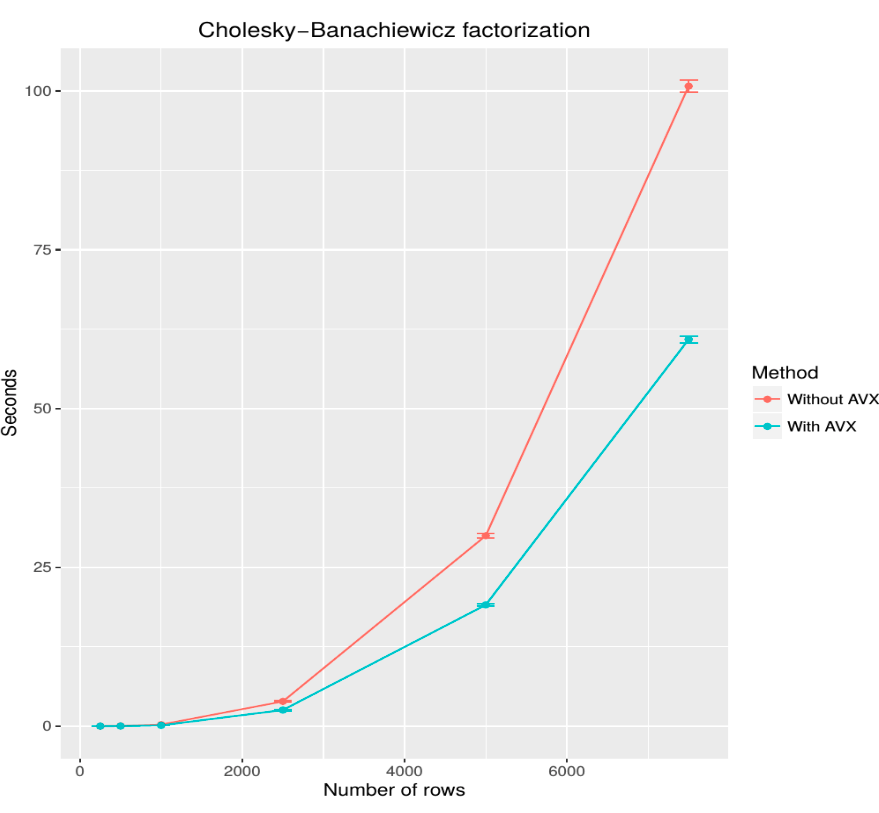
\includegraphics[width=\linewidth]{img/experiment}
  \caption{Comparing the performance of two algorithms}
  \end{center}
\end{figure}

The speedup of this algorithm on the largest matrix is

\[ S_p(n) = \frac{T^{*}(n)}{T_p(n)} = 1.6547 \]

Here $T^{*}(n)$ is the mean time of sequential algorithm and $T_p(n)$ is the mean execution time of the parallel AVX algorithm. This means that the parallel algorithm requires approximately $33\%$ less time than the sequential version.

\section{Comparison to LAPACK and future work}

As a baseline model for my experiments I chose the implementation of Cholesky factorization in LAPACK package which is called by \texttt{chol} function in R. I tested it on the same 6 matrices and the execution time on the largest matrix (7500 rows) was less then 2 seconds. Investigation of the source code of openBLAS\footnote{\url{https://www.openblas.net}} and several papers about LAPACK optimizations\cite{Andersen-2001} tells us that these libraries don't use the iterative Cholesky-Banachiewicz or Crout implementations, but a more complex recursive Cholesky factorization algorithm with a specialized data structure that doesn't store redundant elements of upper triangular matrix.

The goal of my work was to provide a simple demonstration of how AVX instructions can be used to speed up the factorization. It would be interesting though to continue this research and see if similar optimizations can make recursive implementation of LAPACK even faster.

\section{Conclusions}

As we can see, AVX instructions provide a simple way of optimizing algorithms that involve vector or matrix operations. Unlike multithreading, intrinsic operations don't have big latency which allows us to use them even on the small scale.

My implementation of Cholesky factorization was $33\%$ faster than the sequential one. And even though it did not beat the LAPACK implementation, this demonstration of possibilities of AVX instructions shows us one possible way how the most widely used linear algebra packages can be improved.

\bibliographystyle{alpha}
\bibliography{CholeskyAVX}

\end{document}